%Paty projekt do predmetu ITY 2013/2014
%Autor: Lukas Pelanek
%email: xpelan03@stud.fit.vutbr.cz


\documentclass[pdf,slideColor,azure]{prosper}
\usepackage[czech]{babel}
\usepackage{color}
\DefaultTransition{Split}
\usepackage[utf8]{inputenc}
\usepackage{graphics}
\slideCaption{Typografie a publikování \,-\, 5. projekt, Lukáš Pelánek}

\begin{document}

\title{Rafael Nadal}
\subtitle{španělský profesionální tenista}
\author{Lukáš Pelánek}
\email{xpelan03@stud.fit.vutbr.cz}
\date{5. května 2014}
\maketitle

\begin{slide}{Základní informace}	
\begin{itemize}
\item celým jménem Rafael Nadal Parera
\item narozen 3. června 1986 v~Manacoru
\item otec Sebastián Nadal
\item matka María Parera
\begin{figure}
\centering
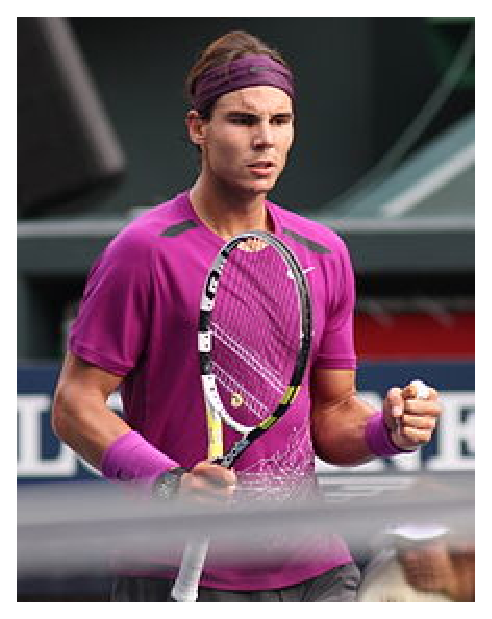
\includegraphics[scale=0.5]{obr1.eps}
\end{figure}
\end{itemize}
\end{slide}

\begin{slide}{Začátky sportovní kariéry}
\begin{itemize}
\item v~8 letech vyhrál regionální turnaj pro hráče do 12 let
\item v~12 letech vyhrával španělské a evropské turnaje ve své věkové kategorii, současně s~tenisem hrál aktivně i fotbal
\item otec ho nechal vybrat mezi tenisem a fotbalem, nakonec zvolil tenis
\item ve věku 15 let se stal profesionálem
\item v~17 letech porazil Rogera Federera a stal se nejmladším hráčem, který se dostal do třetího kola Wimbledonu
\end{itemize}
\end{slide}

\begin{slide}{Profesionální kariéra}
\begin{itemize}
\item v~roce 2005 porazil Mariana Puerta ve finále French Open a stal se tak druhým hráčem po Matsu Wilanderovi, který vyhrál French Open na první pokus
\item v~roce 2008 vyhrál olympijské zlato ve dvouhře a současně ve stejném roce se stal světovou jedničkou
\item v~roce 2010 vyhrál 3 Grand Slamy ze 4
\begin{figure}
\centering
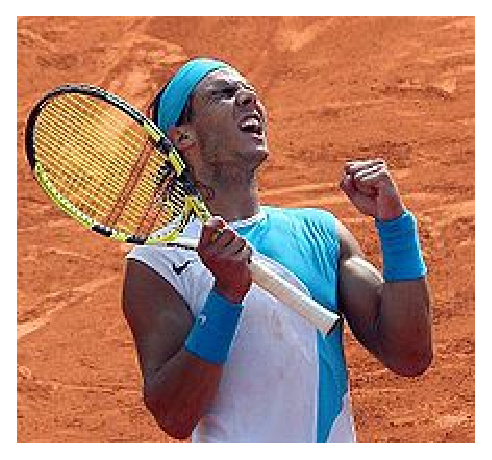
\includegraphics[scale=0.4]{obr2.eps}
\end{figure}
\end{itemize}
\end{slide}

\begin{slide}{Úspěchy}
\begin{itemize}
\item za svoji profesionální kariéru již vyhrál 683 zápasů a 134 prohrál
\item celkem získal 62 titulů, což ho řadí na sedmé místo
\end{itemize}
\begin{table}[hc]
\begin{tabbing}
Australian Open \quad \= 2008 \= 2009 \= 2010 \= 2011 \= 2012 \= 2013  \kill
\textbf{Turnaj} \> 2008 \> 2009 \> 2010 \> 2011 \> 2012 \> 2013 \\
\textbf{Australian Open} \> SF \> V~\> ČF \> ČF \> F \> N \\ 
\textbf{French Open} \> V~\> 4K \> V~\> V~\> V~\> V~\\ 
\textbf{Wimbledon} \> V~\> N \> V~\> F \> 2K \> 1K \\
\textbf{US Open} \> SF \> SF \> V~\> F \> N \> V~\\
\end{tabbing}
\end{table}
V\,-\,vítěz, F\,-\,finále, SF\,-\,semifinále, ČF\,-\,čtvrtfinále, 4K\,-\,4. kolo, 3k\,-\,3. kolo, 2K\,-\,2. kolo, 1K\,-\,1. kolo, N\,-\,nezúčastněn
\end{slide}

\begin{slide}{Rekordy}
\begin{itemize}
\item jako jediný hráč vyhrál 9 po sobě jdoucích let alespoň 1 Grand Slam ročně
\item jako jediný hráč vyhrál 8 krát French Open
\item společně s~Andre Agassim jako jediní dva hráči zkompletovali Golden Slam (výhra na všech Grand Slamech a zisk zlaté medaile z~olympiády)
\item jako jediný hráč vyhrál French Open, Wimbledon a US Open v~jednom kalendářním roce
\item jako jediný hráč získal 26 titulů ze série ATP Masters
\end{itemize}
\end{slide}

\begin{slide}{Rivalita}
\begin{itemize}
\item Nadal vs. Federer
\begin{itemize}
\item odehráli spolu již 33 zápasů, z~nichž 23 vyhrál Nadal
\end{itemize}
\item Nadal vs. Djokovic
\begin{itemize}
\item odehráli spolu již 40 zápasů, z~nichž 22 vyhrál Nadal
\end{itemize}
\item Nadal vs. Murray
\begin{itemize}
\item odehráli spolu již 18 zápasů, z~nichž 13 vyhrál Nadal
\end{itemize}
\begin{figure}
\centering
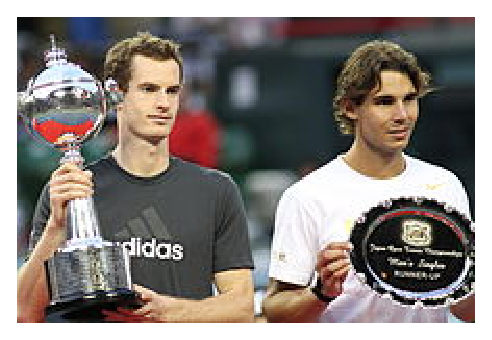
\includegraphics[scale=0.45]{obr3.eps}
\end{figure}
\end{itemize}
\end{slide}

\begin{slide}{Použité zdroje}
\begin{itemize}
\item http://en.wikipedia.org/wiki/Rafael\_Nadal
\end{itemize}
\end{slide}
\end{document}